%%% Local Variables:
%%% TeX-command-extra-options: "-shell-escape"
%%% End:

\section{The base}

\subsection{Containers}

\begin{frame}[fragile]
  \frametitle{Containers}
\begin{figure}[ht]
  \caption{Why Containers}
  \centering
  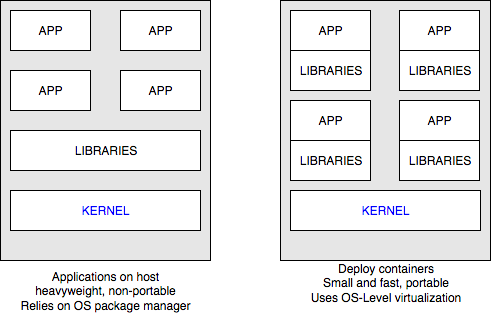
\includegraphics[scale=0.5]{ContainerDiagram.png}
  \label{fig:ContainerDiagram}
\end{figure}
\end{frame}

\subsection{Understanding Pods}

\begin{frame}
  \frametitle{Understanding Pods}
  \begin{itemize}
  \item<1->A \emph{Pod} is the smallest and simplest unit in the Kubernetes object model that we create or deploy.
  \item<2->A Pod represents a running process on our cluster.
    \begin{itemize}
    \item<3->A \emph{Pod} encapsulates an application container (or, in some cases, multiple containers)
    \item<4->A \emph{Pod} storages resources
    \item<5->A \emph{Pod} has an unique network IP
    \end{itemize}
  \item<6->A \emph{Pod} represents an unit of deployment:
  \end{itemize}
\end{frame}

\subsection{Main Ways}

\begin{frame}
  \frametitle{Main ways}
  Pods in a Kubernetes cluster can be used in two main ways:
  \begin{itemize}
  \item<2->Pods that run a single container (most common Kubernetes use case)
  \item<3->Pods that run multiple containers that need to work together(encapsulate an application composed of multiple co-located containers that tightly coupled)
  \end{itemize}
\end{frame}

\subsection{Patterns}

\begin{frame}[fragile]
  \frametitle{Patterns for Composite Containers: Sidecar}
  \begin{figure}[ht]
    \caption{schema of our Sidecar}
    \centering
    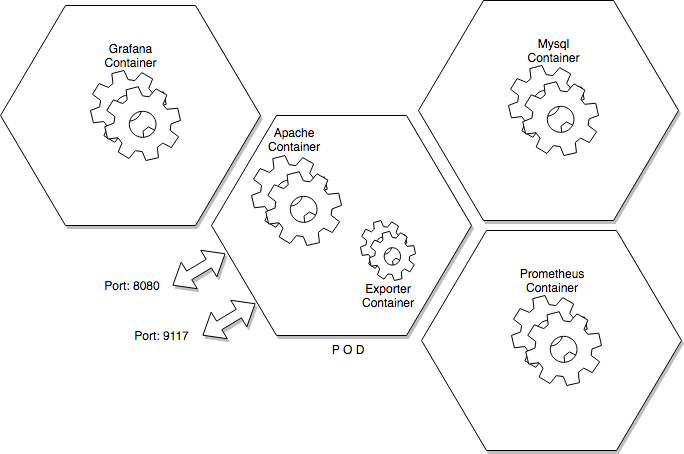
\includegraphics[scale=0.4]{SidecarDiagram.png}
    \label{fig:SidecarDiagram}
  \end{figure}
\end{frame}
